\lab{Application}{Newton's Method}{Newton's Method}
\label{lab:NewtonsMethod}
\objective{Understand Newton's Method}

One important technique in technical computing is Newton's method. The goal of Newton's method is to find $x^*$ such that $f(x^*) = 0$. This method is especially important in optimization, where our goal is to find minima and maxima of functions. Newton's method is an iterative method (much like eigenvalue finders: remember how those provably have to be iterative?). Newton's method, in one dimension, is defined as follows:
\[
x_{n+1} = x_n - \frac{f(x_n)}{f'(x_n)}
\]

Essentially Newton's method approximates a function by its tangent line, and then uses the zero of the tangent line as the next guess for $x_n$.
\begin{figure}[h!]
\begin{center}
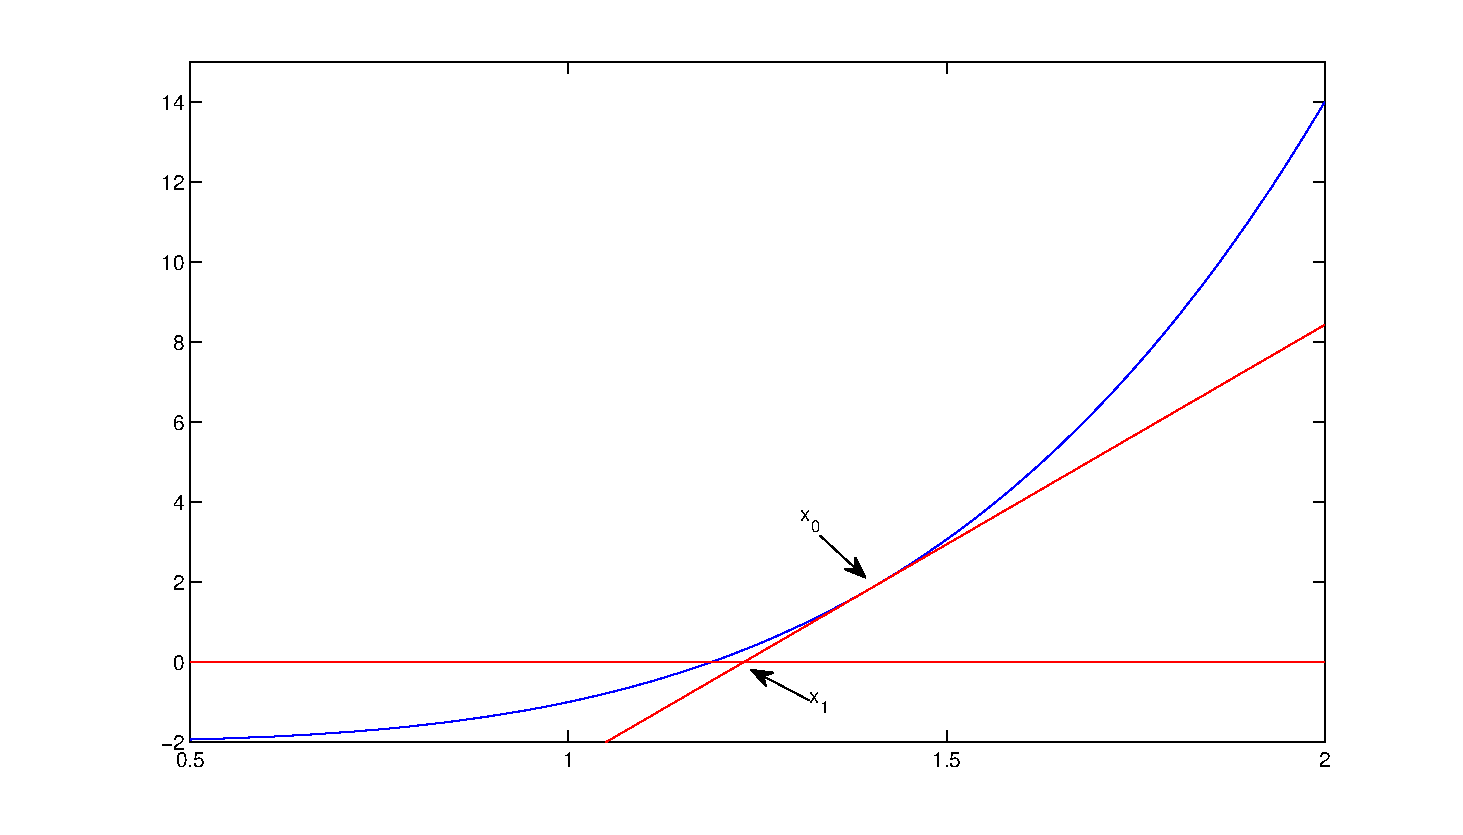
\includegraphics[scale = .5]{newton}
\caption{An illustration of how one iteration of Newton's method works}
\end{center}
\end{figure}

Newton's method is powerful because of the speed of convergence. In many cases Newton's method converges to the actual root quadratically, meaning that the error term is squared at every iteration. This fast convergence makes it a very powerful algorithm.

Newton's method does suffer from the flaw that its convergence is dependent upon an initial guess. If the initial guess is not sufficiently close the convergence can be much slower, or may never occur. There are even certain pathological functions for which newton's method will never converge. However, these functions are very rare, and as a rule Newton's method converges very quickly.



\begin{problem}
Modify the Newton's method function that you wrote in chapter one so that it runs whether or not the user inputs a derivative function. In python this can be done by defining the derivative function as a keyword argument.  Your function definition will look something like this \li{def new_newton(f, x0, df=None, tol=0.001)}

Compare the performance of Newton's method when you input the derivative and when you don't. How well does each converge? Which runs faster? Try the following functions:

\begin{itemize}
\item $cos(x)$
\item $sin(1/x)*x^2$
\item $(sin(x)/x)-x$
\end{itemize}

%When I tested it out in python, hand fed derivatives performed  faster
%cos: 10 times as fast
%sin(1/x)x^2: 7 times as fast
%sin(x)/x - x: 5 times as fast
%sin(x)/x + x: 6 times as fast
%We should specify error bounds and initial guesses for roots
%for some I had trouble with starting guesses producing a zero-valued derivative

%I did not test this in Matlab, and the Matlab version suggests ``$sin(x)/x + x$ might work well.''

\end{problem}

\begin{problem}
Test your newton's method function on $x^{1/3}$. Use random starting points around zero. What do you see? Prove that for any non-zero starting point that newton's method will diverge.
\end{problem}

\begin{problem}
A basin of attraction can be loosely defined as a set that will eventually converge to a specific root. Pick random points on the interval $[-2,2]$ as starting points and apply newton's method to the function $x^3 -2x + 1/2$. Display the basins of attraction for this particular function. What do you observe?

% I don't know anything about attractors, but I graphed mine with the function with these lines
% I thought it helped me visualise it better
% f = lambda x: x**3 - 2*x + 1./2
% df = lambda x: 3*x**2 -2
% x0 = sp.linspace(-2,2,100)
% r = [ newtons2.newtonsMethod(f,df,x,0.001) for x in x0]
% y = [ x**3 - 2*x + 1./2 for x in x0]
% plt.plot(x0,r,x0,y)
% plt.axhline(0,color='black')
% plt.show()

\end{problem}

\begin{problem}
% I found this one very difficult, because scipy does not have a jacobian function, and I kept running into little problems with mine
% However, I did manage to solve it. Perhaps we should supply them a jacobian function
Extend your Newton's method even further so that it will work on systems of equations. Suppose that $F: \mathbb{R}^n \rightarrow \mathbb{R}^n $. The relevant equation is
\[
x_{i+1} = x_i - J^{-1}F(x_i)
\]
Note that you {\bf should not} calculate the inverse Jacobian. \li{sp.solve(A,b)} gives you the solution $x$ to the equation $Ax=b$. Use this fact to calculate $J^{-1}F$ from $J$ and $F$.  You should be able to make this function work whether or not the user inputs a Jacobian. This also means that you will have to implement your own \li{jacobian} function.
\end{problem}

